\documentclass{standalone}
\usepackage{tikz}
\usepackage{xcolor}
\usepackage{amsmath}
\usepackage{amssymb}
\usetikzlibrary{shapes,arrows,positioning,fit,calc,decorations.pathreplacing}

\definecolor{inputcolor}{RGB}{173,216,230}
\definecolor{corecolor}{RGB}{255,218,185}
\definecolor{aggregatecolor}{RGB}{144,238,144}
\definecolor{outputcolor}{RGB}{255,182,193}

\begin{document}

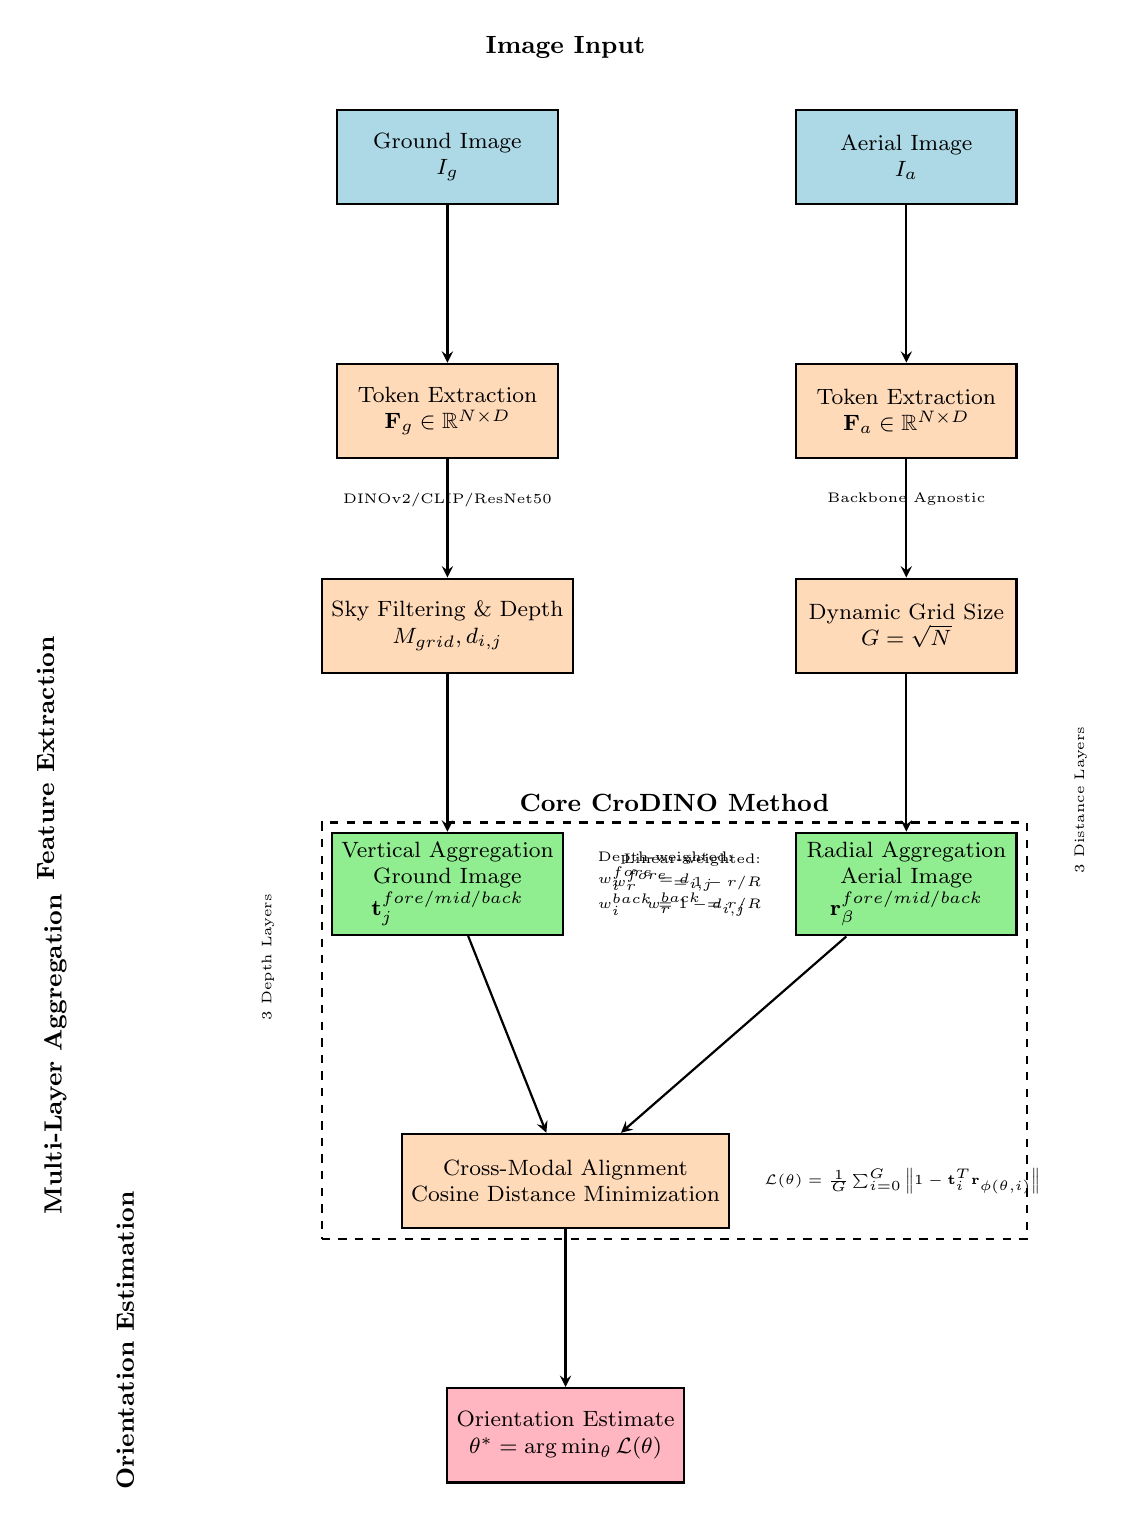
\begin{tikzpicture}[
    node distance=2cm,
    auto,
    thick,
    input/.style={rectangle, draw, font=\footnotesize, align=center, minimum width=2.8cm, minimum height=1.2cm, fill=inputcolor},
    core/.style={rectangle, draw, font=\footnotesize, align=center, minimum width=2.8cm, minimum height=1.2cm, fill=corecolor},
    aggregate/.style={rectangle, draw, font=\footnotesize, align=center, minimum width=2.8cm, minimum height=1.2cm, fill=aggregatecolor},
    output/.style={rectangle, draw, font=\footnotesize, align=center, minimum width=2.8cm, minimum height=1.2cm, fill=outputcolor},
    arrow/.style={->, >=stealth, thick}
]

% Input Images
\node[input] (ground_img) {Ground Image\\$I_g$};
\node[input, right=3cm of ground_img] (aerial_img) {Aerial Image\\$I_a$};

% Feature Extraction (Backbone Agnostic)
\node[core, below=of ground_img] (ground_tokens) {Token Extraction\\$\mathbf{F}_g \in \mathbb{R}^{N \times D}$};
\node[core, below=of aerial_img] (aerial_tokens) {Token Extraction\\$\mathbf{F}_a \in \mathbb{R}^{N \times D}$};

% Key Processing Steps
\node[core, below=1.5cm of ground_tokens] (preprocessing) {Sky Filtering \& Depth\\$M_{grid}, d_{i,j}$};
\node[core, below=1.5cm of aerial_tokens] (grid_calc) {Dynamic Grid Size\\$G = \sqrt{N}$};

% Core Aggregation
\node[aggregate, below=2cm of preprocessing] (vertical_agg) {Vertical Aggregation\\Ground Image\\$\mathbf{t}_j^{fore/mid/back}$};
\node[aggregate, below=2cm of grid_calc] (radial_agg) {Radial Aggregation\\Aerial Image\\$\mathbf{r}_\beta^{fore/mid/back}$};

% Core Method - Orientation Estimation
\node[core, below=2.5cm of vertical_agg, xshift=1.5cm] (alignment) {Cross-Modal Alignment\\Cosine Distance Minimization};

% Output
\node[output, below=2cm of alignment] (orientation) {Orientation Estimate\\$\theta^* = \arg\min_\theta \mathcal{L}(\theta)$};

% Arrows
\draw[arrow] (ground_img) -- (ground_tokens);
\draw[arrow] (aerial_img) -- (aerial_tokens);
\draw[arrow] (ground_tokens) -- (preprocessing);
\draw[arrow] (aerial_tokens) -- (grid_calc);
\draw[arrow] (preprocessing) -- (vertical_agg);
\draw[arrow] (grid_calc) -- (radial_agg);
\draw[arrow] (vertical_agg) -- (alignment);
\draw[arrow] (radial_agg) -- (alignment);
\draw[arrow] (alignment) -- (orientation);

% Key Innovation Highlight
\node[draw, dashed, thick, fit={(vertical_agg) (radial_agg) (alignment)}, 
      label={[font=\small\bfseries]above:Core CroDINO Method}] {};

% Mathematical Annotations
\node[right=0.3cm of vertical_agg, font=\tiny, align=left] {
    Depth-weighted:\\
    $w_i^{fore} = d_{i,j}$\\
    $w_i^{back} = 1-d_{i,j}$
};

\node[left=0.3cm of radial_agg, font=\tiny, align=right] {
    Linear-weighted:\\
    $w_r^{fore} = 1-r/R$\\
    $w_r^{back} = r/R$
};

\node[right=0.3cm of alignment, font=\tiny, align=left] {
    $\mathcal{L}(\theta) = \frac{1}{G} \sum_{i=0}^{G} \left\| 1 - \mathbf{t}_i^T \mathbf{r}_{\phi(\theta,i)} \right\|$
};

% Backbone Flexibility Note
\node[below=0.3cm of ground_tokens, font=\tiny] {DINOv2/CLIP/ResNet50};
\node[below=0.3cm of aerial_tokens, font=\tiny] {Backbone Agnostic};

% Layer Annotation
\node[left=0.8cm of vertical_agg, font=\tiny, rotate=90] {3 Depth Layers};
\node[right=0.8cm of radial_agg, font=\tiny, rotate=90] {3 Distance Layers};

% Phase Labels
\node[above=0.5cm of ground_img, font=\small\bfseries, xshift=1.5cm] {Image Input};
\node[left=3.5cm of preprocessing, font=\small\bfseries, rotate=90] {Feature Extraction};
\node[left=3.5cm of vertical_agg, font=\small\bfseries, rotate=90] {Multi-Layer Aggregation};
\node[left=3.5cm of alignment, font=\small\bfseries, rotate=90] {Orientation Estimation};

\end{tikzpicture}

\end{document}
